\section{Empirical study}

We studied the DIM with four text corpora: three collections of
scientific articles and a collection of opinions written by judges in
the New York Appellate Court system.  For each corpus, we estimated
and examined the posterior distributions of its articles' influence.

In this section, we demonstrate that the estimate of an article's
influence is robustly correlated to the number of citations it
received.  While the DIM model is designed for corpora without
citations---and, indeed, only the documents' text and dates are used
in fitting the model---citations remain an established measure of
influence.  This study provides validation of the DIM as an
exploratory tool of influential articles.

% dmb: not an svn error: i re-added the sentence above.  i liked it.

% We also provide several examples to demonstrate that this model
% provides a bibliometric similar to citations with distinctive
% qualities.

\subsection*{Data}
\label{sec:data}

% dmb: put this fact somewhere else.  did inference take the same
% amount of time for each corpus?

% smg: it was close, with nature taking a little longer.  I don't know
% where else it belongs, so I'll leave it out.

% dmb: well, it's nice to give an example of how long inference takes.
% i think it's okay to say something like "to give a sense for how
% long the algorithm takes, the XXX corpus with XXX topics took XXX
% time to converge on an XXX machine."  also, i suggest briefly adding
% details like the variational convergence criterion and how the model
% is initialized.  (no need to report sensitivity, just give the facts
% so that someone can replicate our experiments.)

% smg: re-added, below.
% 

The three scientific corpora we analyzed were the \emph{ACL
  Anthology}, \emph{The Proceedings of the National Academy of
  Science}, and the journal \emph{Nature} (we discuss the New York
Courts in a later section).  For each corpus, we removed short
documents, terms that occurred in too few documents, and terms that
occurred in too many documents.  We also removed terms whose
statistics did not vary over the course of the collection, as such
terms would not be useful for assessing change in language (a sample
of such non-varying terms from \emph{Nature} is ``ordinarily'',
``shake'', ``centimetre'', ``traffic'', and ``themselves'').

\textbf{ACL Anthology.} The \emph{Association for Computational
  Linguistics Anthology} is a digital collection of publications about
computational linguistics and natural language
processing~\citep{bird:2008}.  We analyzed a 50\% sample from this
anthology, spanning 1964 to 2002.  Our sample contains 7,561
articles and 11,763 unique terms after preprocessing.  For this corpus
we used article citation counts from the \emph{ACL Anthology
  Network}~\citep{Radev:2009}.

\textbf{PNAS.} The \emph{Proceedings of the National Academy of
  Sciences} is a leading, highly-cited, multidisciplinary scientific
journal covering biological, physical, and social sciences.  We
sampled one seventh of the collection, spanning 1914 (when it was
founded) to 2004.  Our sample contains 12,145 articles and 14,504
distinct terms after preprocessing.  We found citations using Google
Scholar for 78\% of this collection.

\textbf{Nature.} The journal \emph{Nature} is the world's most highly
cited interdisciplinary science journal~\citep{Thompson:2009} with
content on a range of scientific fields. We analyzed a $10\%$
sample from this corpus, spanning 1869 (when it was founded) to
2008.  Our sample contains 34,418 articles and 6,125 distinct terms
after preprocessing.  We found citations using Google Scholar for 31\%
of these documents.

% smg: Note that this will make us run out of space.
Inference for 10 topics on each corpus above took about 11 hours to
converge on a desktop Intel 2.4GHz Core 2 Quad cpu.  Our convergence
criterion was met when the evidence lower bound increased by no more
than 0.01\%.  For the experiments described below, we set topics'
Markov chain variance $\sigma^2=0.005$ and $\sigma_d=\sigma_l=0.0001$.


% \begin{figure}
%  \small
% \begin{centering}
%   \caption{Preprocessing thresholds for each corpus.}
%   \begin{tabular}{|l|l|l|l|}
%     \hline
%     Minimum fraction of documents & 0.2\% & 0.4\% & 0.3\% \\
%     Maximum fraction of documents & 25\% & 15\% & 20\% \\
%     Maximum fraction of documents &      &      &      \\
%     in any year & 40\%& 30\% & 40\% \\
%     Minimum stdandard deviation & 0.75 & 1.2 & 1.5 \\
%     \hline
%     & \emph{Nature} & \emph{PNAS} & \emph{ACL} \\
%     \hline
%   \end{tabular}
%   \label{fig:preprocess_thresholds}
%   \end{centering}
%   \normalsize
%     \vspace{-10pt} \\
% \end{figure}

\subsection*{Relating posterior influence and citation}
\label{sec:results}

We studied the DIM with varying numbers of topics.  We measured the
relationship between the posterior influence values of each article
$\ellv_d$ and its citation count $c_d$.

We first aggregate the influence values across topics.  Recall that
each document has an influence value for each topic.  For each word,
we compute its expected posterior influence score, with the
expectation taken with respect to its (random) topic assignment.  We
then sum these values over all words in the document,
\begin{equation}
  f(\ellv_d) = \sum_{n=1}^{N_d} \textrm{E}[z_{d,n} \cdot \ellv_d].
  \label{eq:score}
\end{equation}
This weights each word by the influence associated with its assigned
topic.  (Using the maximum value of influence across topics yielded
similar results.)

% dmb: below, i commented out this paragraph.  this seemed like it
% shouldn't be there anymore since you added a part about the new
% metric.  that said, perhaps you should add a point about taking
% correlation to log, if that is still what we're doing.

% \paragraph{Metrics.}  We used two metrics to measure the relationship
% between the aggregated influence scores and citations.  First, we
% computed the correlation between influence score and $\log(c_d + 1)$,
% which provides a commonly understood test statistic.  We take the log
% to account for overdispersion---once an article is cited, it is likely
% to be cited more.  We also 

%Second, we compute a metric, the standardized median deviation, on the
%first fifty most influential articles.  (Our idea is that this is a
%reasonable number for a scientist to examine.)  First, we standardize
%the log citations, computing for each article the number of standard
%deviations from the mean of the log citations.  This step is taken to
%make this metric comparable across datasets that have different
%numbers of citations.  We then select the top 50 documents $\{
%d_{i_1}, \ldots, d_{i_{50}} \}$ by their aggregate posterior influence
%and compute the median standardized citation of them.  This provides a
%robust indication of the model's performance on its top documents; the
%typical article will have value 0, and a bad article will have a
%negative value.

% dmb: has the idea of the influence envelope been added to the
% modeling section?  it should be...

% smg: Yes, I moved it there in the earlier revision.

% \paragraph{Influence envelope}
% One might expect that documents tend to have greatest influence
% shortly after publishing; indeed, the median number of citations to
% scientific articles begins decreasing within 10 years
% \cite{porter:2005}.  One parameter in the model determines the amount
% of influence an article has after $n$ years
% \begin{align*}
%   \textstyle r_n(t) = \left\{
%     \begin{array}{ll}
%       \frac{1}{n} & t <= n  \\
%       0 & t >= n
%     \end{array} \right., t = 0, 1, 2, \ldots,
% \end{align*}
% where we refer to $r_n$ as the \emph{influence envelope} of length $n$. While
% this envelope is discontinuous and arguably unnatural, it remains
% simple and provides useful information about the model. Across all
% corpora, we found that shorter envelopes yield a closer
% relationship between our model and citations.

\begin{figure*}[t]
  \centering
  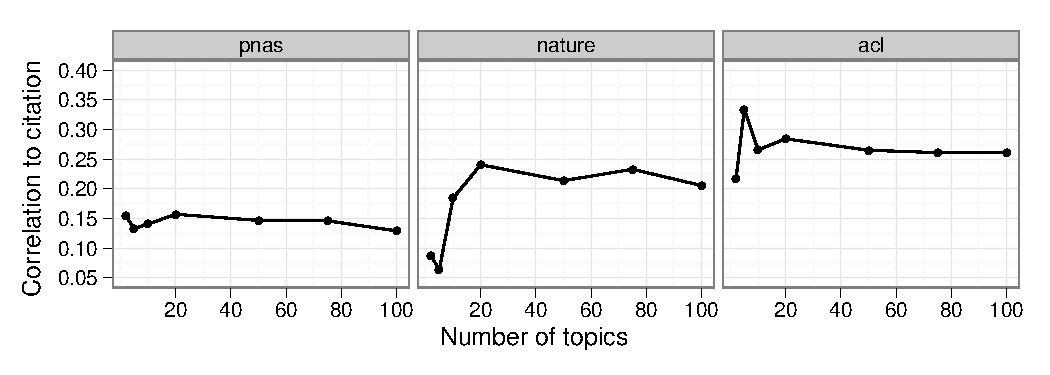
\includegraphics[width=0.8\textwidth]{chapter_influence/figures/results_correlation.pdf} \\
  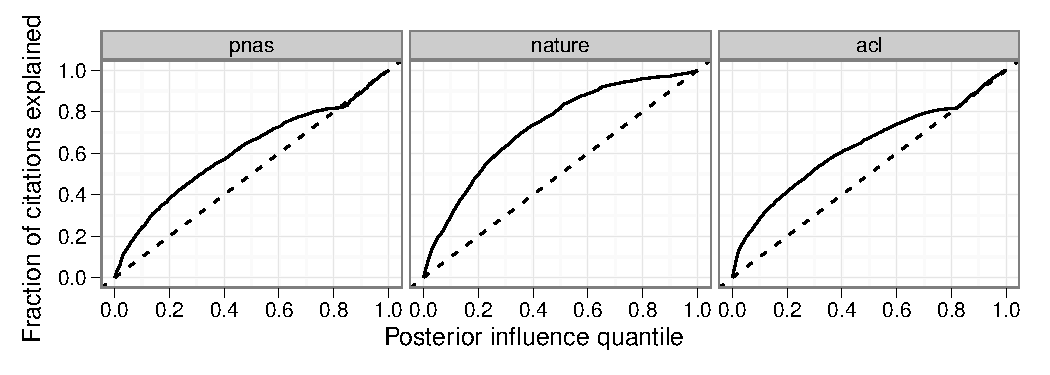
\includegraphics[width=0.8\textwidth]{chapter_influence/figures/results_roc.pdf} \\
  \caption{Spearman rank correlation between citation counts and
    posterior influence score, controlling for date (top) and fraction
    of citations explained by posterior influence (bottom).}
  \label{fig:results}
\end{figure*}

\myfig{results} displays the Spearman rank correlation between the
aggregated posterior influence score of \myeq{score} and citation
counts.  The DIM posterior---which is estimated only from the texts of
the articles---has a positive correlation to the number of citations.
All of these numbers were found significant up to $p<1e-4$, using
permutation tests on the influence scores.

Correlation goes up when we model multiple topics within a corpus.
Moving from 2 to 5 topics in the \emph{ACL} corpus increases
correlation from 0.25 to 0.37.  \emph{Nature} is likewise better with
more topics, with a correlation of 0.28 at 20 topics; while
\emph{PNAS} performs best near 5 topics, with a correlation of 0.20.

% These numbers make sense: the \emph{ACL} corpus is much more
% specialized than \emph{Nature}, so more topics are required to
% discriminate research fields for Nature.

\myfig{results} also shows the fraction of citations explained
by DIM scores: \emph{Nature} documents with the highest 20\% of
posterior influence, for example, received 56\% of citations.  The
flat regions in \emph{ACL} and \emph{PNAS} are due to aggregate
influence scores very close to zero.

% dmb: see my comment above: has the idea of the influence envelope
% been added to the modeling section?
% smg: It should be (provided that there wasn't an svn issue)

% All numbers reported above and plotted use flat influence envelopes of
% 4 years for each of \emph{ACL} and \emph{PNAS} and 10 years for
% \emph{Nature}. We found empirically that small windows of influence
% are most highly correlated with citations, suggesting that the added
% complexity of the larger windows may not be justified.

% dmb: this feels like too much detail.  if a reviewer asks about it,
% we can mention it.  did we end up with random restarts?

% smg: for most of the data, it was random.  for the last set of
% experiments (not included), it wsa not.

% Selecting the correct number of topics is important for the model
% because it defines the granularity at which the model identifies
% influence.  Further, different topics may be found when topics are
% initialized with different random seeds. That said, we still find
% high correlation in results with different initializations and
% differing numbers of topics.  In a 50-topic model vs. a 75-topic
% model over \emph{Nature}, for example, the correlation coefficient
% of documents' posterior influence is 0.72.

\paragraph{Heuristic model.} 
 The DIM is a complicated model. To
justify its complexity, we describe a simple baseline (the
\emph{heuristic}) which captures our intuition with a single topic, is
easy to implement, and runs quickly.  For this heuristic, we define a
word's weight at time $t$ as:
\[
w_t := \textstyle \frac{\mbox{Frequency of } w \mbox{ in } [t, t + f] }
{\mbox{Frequency of }w \mbox{ in }[t - p, t]
},
\]
for fixed distances $f$ into the future and $p$ into the past.
A document's score is the weighted average of its words'
weights. This heuristic captures the intuition that influential
documents use language adopted by other documents.

% dmb: i'm confused which results are being reported below.  first we
% say that "the model with a single topic generally outperforms the
% heuristic."  then we say "however" the heuristic performs well with
% large values of the parameters.

The heuristic performed best with large values of its parameters
($f=p=200$). With these settings, it achieves a correlation of 0.20 for
the \emph{ACL}, 0.20 for \emph{PNAS}, and 0.26 for \emph{Nature}.  For
\emph{Nature}, the model is more correlated with citations than the
heuristic for 20, 50, and 75 topics.  Correlation is matched for
\emph{PNAS}, the model slightly beating the heuristic at 5 topics.
\emph{ACL} outperforms the heuristic for all numbers of topics.

\paragraph{Shuffled corpus} Though we have eliminated date as a
confounder by controlling for it in correlations, there may be other
confounders such as document length or topic distribution.  We
therefore measured the DIM's relationship to citations when dates were
randomly shuffled, keeping all documents which share a date
together. If non-date confounders exist, then we might see correlation
in the shuffled data, marking observed correlation as dubious.

We shuffled dates in the corpora and refit the DIM.  We found a
\emph{maximum} date-controlled correlation of 0.018 for 29 shuffles of
\emph{ACL}; 0.001 for 5 shuffles of \emph{Nature}; and 0.012 for 28
shuffles of \emph{PNAS}. While this shuffled experiment and
controlling for date do not entirely preclude confounding, they eliminate many
potential confounders.

\subsection*{A closer look}
Experiments showing correlation with citations demonstrate consistency
with existing bibliometrics. However, the DIM also finds qualitatively
different articles than a bibliometric based on citation counts
finds. In this section we describe several documents to give the
reader an intuition behind the kind of analysis that the DIM provides.

\paragraph{IBM Model 3} The second-most cited article in the \emph{ACL
  Anthology Network} is \emph{The Mathematics of Statistical Machine
  Translation: Parameter Estimation}~\citep{brown:1993}. It has 450
intra-\emph{ACL} citations and 2,130 total citations listed on Google
Scholar.  This seminal work describes parameter estimation for five
word-based statistical models of machine translation; it provided
widely accepted statistical models for word alignment and introduced
the well-known ``IBM models'' for machine translation. The posterior
influence score for \cite{brown:1993} ranked $6$ out of 7,561   %  citet
articles in a 10-topic model.

%Figure~\ref{fig:topics} (top) shows a topic discovered by the DIM
%in which \cite{brown:1993} was the most influential over 40 years:
This article was most influential in a topic about translation, which
had a trend toward ``alignment for machine translation.''  The
largest-moving words are shown in \myfig{words} (left).
Upward trends for ``alignment'', ``brown'', and ``equation'' are
evident (although it is not clear whether ``brown'' refers to the
author or the corpus).

% dmb: below, how many intra-acl citations are there?
\paragraph{The Penn Treebank}
The most-cited article in our subset of the \emph{ACL Anthology
  Network} is \emph{Building a large annotated corpus of English: the
  Penn Treebank} \citep{marcus:1993}, with 1,622 \emph{ACL} citations
and 2,810 citations on Google Scholar.  This article describes the
large-scale part-of-speech and syntax tagging of a 4.5-million word
corpus.  It falls in a topic about part-of-speech tagging and syntax
trees; ``treebank'' had become one of the top words in the topic by
2004.

The DIM assigned a relatively low influence score to this article,
ranking it 2,569 out of 7,561 articles.  While \cite{marcus:1993}  % citet
introduces a powerful \emph{resource}, most of the article uses
conventional language and ideas to detail the annotation of the Penn
Treebank.  As such, the paper does not discuss paradigm-changing ideas
and the model scores it low.  We emphasize that this does not
undermine the tremendous influence that the Penn Treebank has had on
the field of natural language processing.  The DIM is not designed to
discover this kind of influence.

% dmb: below, remind us 1st out of how many articles?
% smg: Added 34,418.
\begin{figure*}
  \center
\normalsize
\begin{tabular}{c}
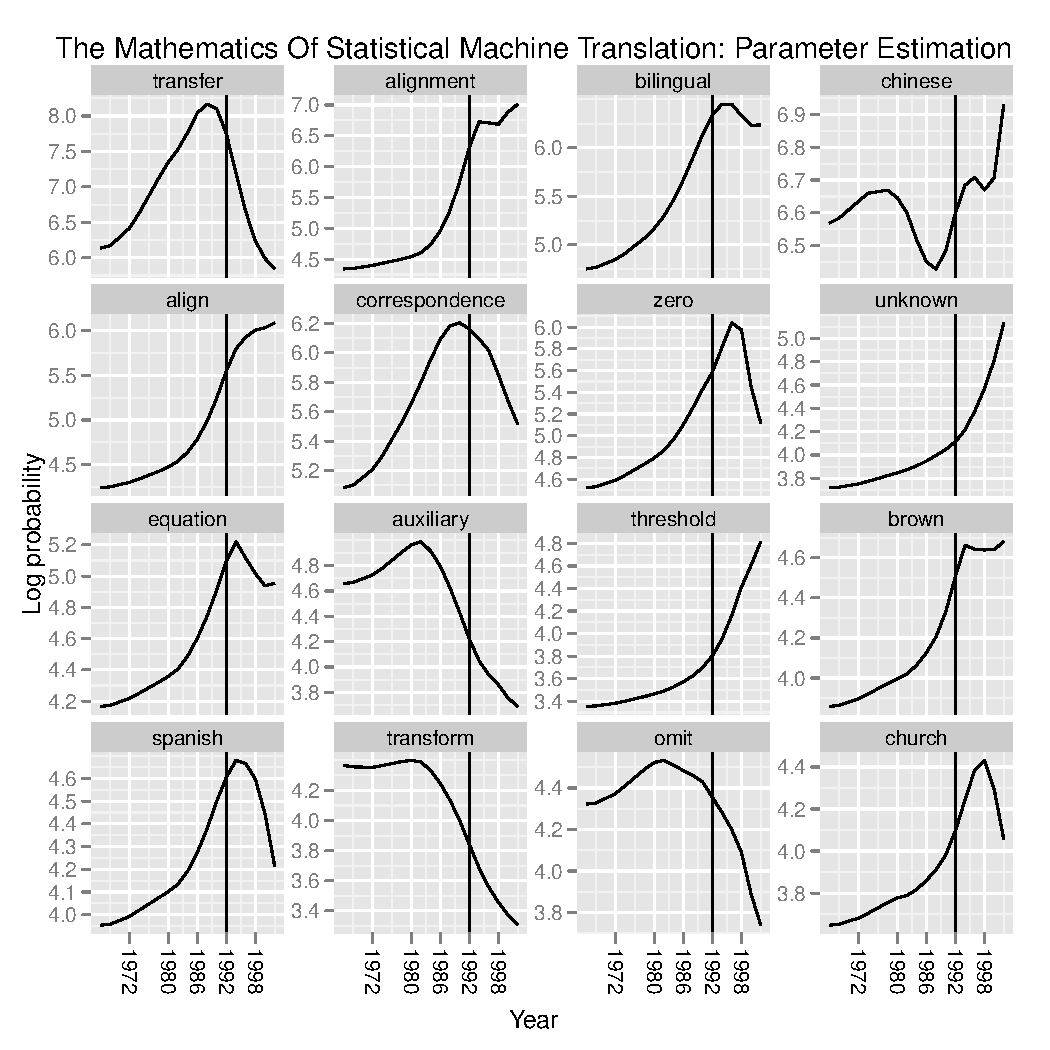
\includegraphics[width=0.7\textwidth]{chapter_influence/figures/acl_brown.pdf}
\\
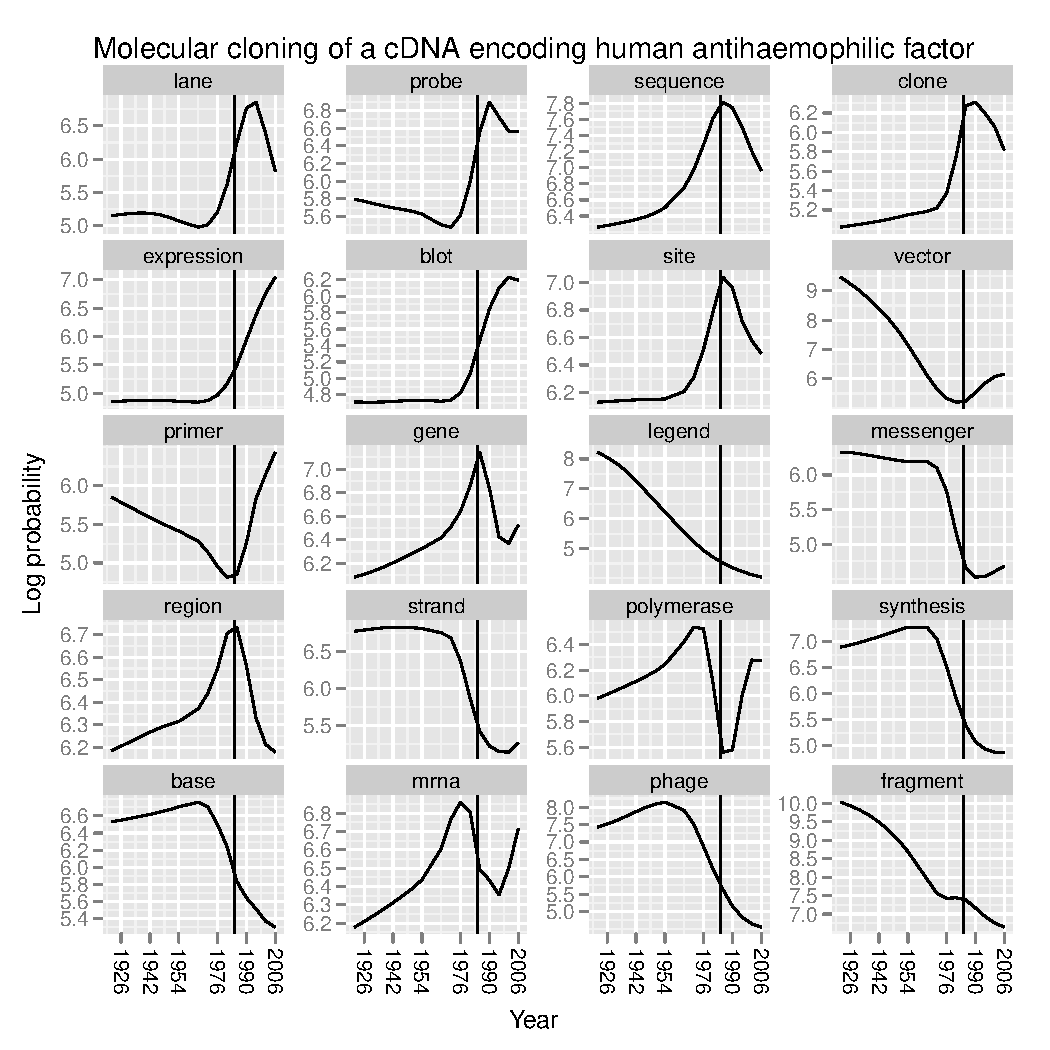
\includegraphics[width=0.7\textwidth]{chapter_influence/figures/nature_cloning.pdf} \\
\end{tabular}
  \small
\caption{Most active words appearing in \cite{brown:1993} (left) which
  have changed the most in a topic about translation. On right are
  words appearing in \cite{toole:1984} in a topic about DNA and
  genetics.  Terms are sorted by increase over 10 years.}  \normalsize
%\label{fig:acl_brown_words}
%\label{fig:nature_cloning}
\label{fig:words}
\end{figure*}

\paragraph{Success in 1972}
In 1967, The College Science Improvement Program was established to
assist predominantly undergraduate institutions.  Two years later
\emph{Nature} published a short column, which has the highest of our
posterior influence in a 20-topic model, out of 34,418 \emph{Nature}
articles.  No citation information was available about this article in
Google Scholar. The column, \emph{How to be Overtaken by Success},
discusses a debate about the ``Miller bill'', which considers funding
for postgraduate education
\citep{Nature.success:1969}. \textit{Overtaken by Success} provides few
research resources to researchers, which may explain lack of citation
information. Instead, it presciently discusses a paradigm shift in a
topic about science, industry, research, and education: ''The record
of the hearings [on the bill] is not merely an indication of the way
the wind is blowing but an important guide to some of the strains
which are now accumulating within the system of higher education...''

In 1972, three years after this article's publication, The NSF
Authorization Act of 1973 made the NSF explicitly responsible for
science education programs \emph{at all levels}
\citep{NSF.website:2010}.  Where this may have been missed by those
using citation counts to study the history of science education, the
DIM has provided a metric with which to gauge interest in the article.

% dmb: again, remind us out of how many articles.
% smg: Done.

\paragraph{Genetics in \emph{Nature}}
The sixth most influential document by the DIM in a 20-topic model of
\emph{Nature} is \emph{Molecular cloning of a cDNA encoding human
  antihaemophilic factor}, an article describing successful
cloning of a human mRNA sequence important in blood clotting
\citep{toole:1984}.  With 584 citations, this article is among the top
0.2\% of these 34,418 documents.  The most active words
appearing in this article are shown in
\myfig{words} (right).  The plot shows some of the
document's key words -- ``expression'', ``primer'', ``blot'' -- become
prominent words in the topic.

\subsection{An application to the New York Appellate Courts.}

The New York Appellate Court system hears appeals cases within the
state of New York.  This court ``was established to articulate
statewide principles of law in the context of deciding particular
lawsuits.''  \citep{nyca_webpage:2012}, acting as a form of ``Supreme
Court'' for the state of New York.  Judges who hear these cases make
decisions about the cases and write opinions summarizing their
reasoning for these decisions.  These decisions and opinions are
extremely important within the court system because they set precedent
for later decisions.

These opinions written by judges are therefore written expressly to be
\emph{influential} on later court decisions, and judges' opinions
frequently make explicit citations to earlier cases.  However, these
citations are limited in two respects.  First, multiple opinions may
exist per case, stating the majority opinion, supporting it in part,
or entirely disagreeing with it. Although judges' citations are
explicit and well-formatted, their citations do not make this
distinction machine-readable, making large-scale analyses difficult
without expensive hand-coding. Second, lawmakers may have different
reasons for citing opinions; it has been hypothesized by some
political methodologists that researchers do not cite dissenting
opinions because dissenting opinions are considered to hold little if
any legal sway; citing dissenting opinions is therefore seen as a sign
of weakness \citep{beim:2011}.

We analyzed this collection, splitting 9,266 appellate court cases into
10,618 distinct opinions, written by judges representing the majority
opinion, a concurrance in part (i.e., supporting the majority decision
but with a different rationale for reaching that decision), or a
dissenting opionion.  Our collection contained 13,568 distinct terms
after pre-processing. We also scraped citations within this collection
and found 37,348 intra-corpus citations.

% pwd
% /n/fs/grash-model/users/sgerrish/nyc_appellate/kq_NYCtApp
 % cat sgerrish/data/v1.9/v1.9-docs.dat | head
 % cat sgerrish/data/v1.9/v1.9-docs.dat | cut -f1 -d_
 % cat sgerrish/data/v1.9/v1.9-docs.dat | cut -f1 -d_ | sort | uniq | wc -l
 % cat sgerrish/data/v1.9/v1.9-docs.dat | cut -f1 -d, | sort | uniq | wc -l
 % cat sgerrish/data/v1.9/v1.9-docs.dat | less
 % ls -lrt sgerrish/src/generate/v1.9/ROADMAP
 % less sgerrish/src/generate/v1.9/ROADMAP
 % wc -l sgerrish/data/v1.8/vocab_filtered_v1.8.txt 
 % less sgerrish/data/v1.9/citation_counts.csv 
 % cat sgerrish/data/v1.9/citation_counts.csv | cut -f2 -d, | awk 'BEGIN{a=0}{a = a + $1}'
 % cat sgerrish/data/v1.9/citation_counts.csv | cut -f2 -d, | awk 'BEGIN{a=0}{a = a + $1}END{print a}'

Based on the analysis of the scientific corpora, we fit a 40-topic
model to this collection to discover influential documents.
Consistent with the scientific corpora, we measured a Spearman
rank-correlation coefficient between posterior influence scores and
the logarithm of citation counts at $\rho=0.24$.  We illustrate the
fraction of citations explained by documents above different influence
thresholds in \myfig{nyca_citations_explained}.  Across all four
corpora, the model is consistently correlated with citation counts.

\begin{figure}
  \center
  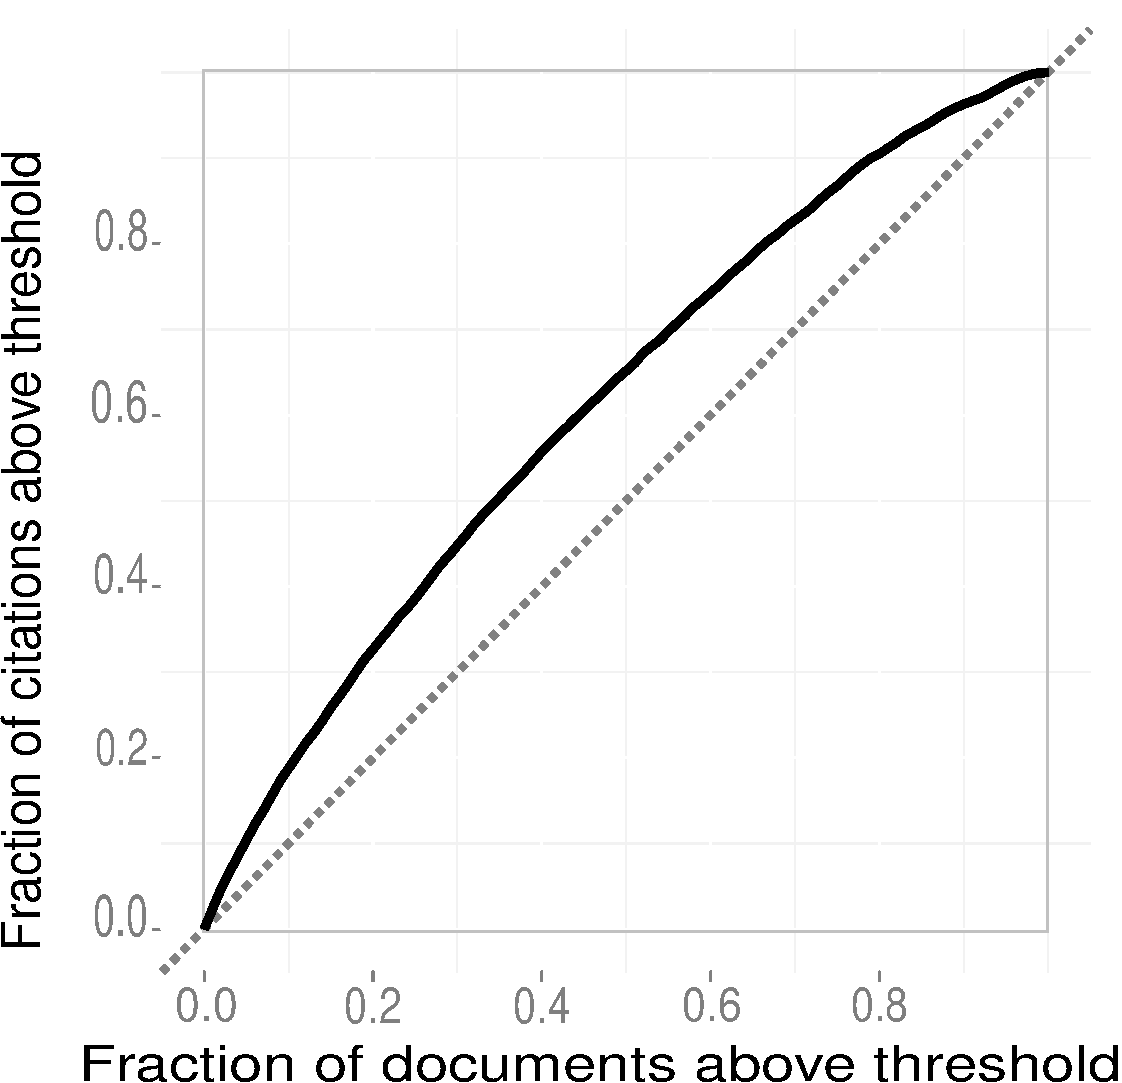
\includegraphics[width=0.4\textwidth]{chapter_influence/figures/fraction_docs_vs_fraction_citations.pdf}
  \caption{Citations explained by influence score in the New York Appellate Courts.  Each point on the curve represents a different threshold of the influence score.  The x-axis describes threshold on the influence score, and the y-axis describes the fraction of citations for all documents which fall below this threshold.}
  \label{fig:nyca_citations_explained}
\end{figure}



% \paragraph{The Cardozo Topic.} Judge Benjamin Cardozo (later Justice
% Cardozo) was one of the most well-known judges in American political
% history.  Cardozo is known for his thoughtful, deliberate opinions and
% is considered to have had an outsize influence on judicial thought.
% One of the more interesting topics discovered by our model in this
% collection identified language which was predominantjuly used by Judge
% Benjamin Cardozo.\footnote{A similar topic was discovered by a dynamic
%   topic model.}  This topic used phrases such as xxx, xxx, and
% xxx. The average ...
 